\documentclass[10pt,letterpaper]{article}
\usepackage[top=0.85in,left=2.75in,footskip=0.75in,marginparwidth=2in]{geometry}

% use Unicode characters - try changing the option if you run into troubles with special characters (e.g. umlauts)
\usepackage[utf8]{inputenc}

% clean citations
\usepackage{cite}

% chemical formula
\usepackage{chemformula}

% SI units
\usepackage{siunitx}
\DeclareSIUnit{\molar}{M}

% hyperref makes references clicky. use \url{www.example.com} or \href{www.example.com}{description} to add a clicky url
\usepackage{nameref,hyperref}

% line numbers
\usepackage[right]{lineno}

% improves typesetting in LaTeX
\usepackage{microtype}
\DisableLigatures[f]{encoding = *, family = * }

% text layout - change as needed
\raggedright
\setlength{\parindent}{0.5cm}
\textwidth 5.25in 
\textheight 8.75in

% use adjustwidth environment to exceed text width (see examples in text)
\usepackage{changepage}

% adjust caption style
\usepackage[aboveskip=1pt,labelfont=bf,labelsep=period,singlelinecheck=off]{caption}

% remove brackets from references
\makeatletter
\renewcommand{\@biblabel}[1]{\quad#1.}
\makeatother

% headrule, footrule and page numbers
\usepackage{lastpage,fancyhdr,graphicx}
\usepackage{epstopdf}
\pagestyle{myheadings}
\pagestyle{fancy}
\fancyhf{}
\rfoot{\thepage/\pageref{LastPage}}
\renewcommand{\footrule}{\hrule height 2pt \vspace{2mm}}
\fancyheadoffset[L]{2.25in}
\fancyfootoffset[L]{2.25in}

% use \textcolor{color}{text} for colored text (e.g. highlight to-do areas)
\usepackage{color}

% define custom colors (this one is for figure captions)
\definecolor{Gray}{gray}{.25}

% this is required to include graphics
\usepackage{graphicx}
\usepackage{subcaption}

% use if you want to put caption to the side of the figure - see example in text
\usepackage{sidecap}

% use for have text wrap around figures
\usepackage{wrapfig}
\usepackage[pscoord]{eso-pic}
\usepackage[fulladjust]{marginnote}
\reversemarginpar

% document begins here
\begin{document}
\vspace*{0.35in}

% title goes here:
\begin{flushleft}
{\Large
\textbf{\newline{Assessing Population Genetics Evidence for Local Adaptation to Phosphorus Availability in Maize.}
}
}
\bigskip
% authors go here:

\textbf{Doctoral Project Proposal} \\
Fausto Villafrade Rodríguez Zapata. M.Sc. 
\bigskip

\textbf{Thesis directors:} \\
Dr. Andrés Moreno Estrada.\\
Dr. Ruben Rellán Álvarez.

\bigskip
\textbf{Committee:}\\
Dr. Alexander de Luna \\
Dr. Luis Delaye Arredondo \\
Dr. Sean Michael Rovito  \\
Dr. Tania Hernández Hernández
\end{flushleft}

\section*{Abstract}
Plant phosphorus starving response (PSR) is a coordinated set of biochemical, physiological and developmental reactions to low phosphorus supply. I expect divergent selection in the genes involved in PSR if it is the result of local adaptation. Given the absence of opposing evolutionary forces, the main consequence of this selection is an increased frequency of adaptive alleles in populations exposed to low phosphorus availability. Here I use a reverse ecology approach to identify PSR genes that might be subject to divergent selection, and to postulate phenotypes relevant to local adaptation. First I built soilP, an R package for assigning soil phosphorus retention potential to geographic locations. Then I performed environmental GWAS on georeferenced genotypes for \textit{Zea mays}. Finally, I propose Qst/Fst analysis and QTL mapping on segregating populations as the next logical steps of my research.


% now start line numbers
\linenumbers

% the * after section prevents numbering
\section*{Introduction}

\paragraph{Phosphorus as limiting nutrient.} 

Different soil phosphorus compounds can be sorted into separate pools according their availability for direct plant use. The most readily available form for plants is Pi in aqueous solution. Next, is the phosphorus in organic compounds, such as nucleotides, phospholipids, phosphorylated sugars and proteins, from which phosphates can be hydrolyzed by enzymatic activity. After this, the non-occluded P fraction that corresponds to phosphate adsorbed to the surfaces of iron and aluminium oxides and \ch{CaCO3} \cite{WALKER19761}. One step less available is the occluded P fraction, that is, phosphate physically encapsulated or surrounded by secondary minerals, such as Fe, Al and Mn oxyhydroxides \cite{Yang:2013ft,Filipelli:6Zj8wyph} by coprecipitation or diffusive penetration \cite{WALKER19761}. Thus the labile, i.e. more bioavailable \cite{Yang:2013ft}, phosphorus pool includes phosphate ions in solution as well as P incorporated in soil organic matter, and to a lesser degree the non-occluded P fraction. The refractory forms, which are not readily bioavailable, include P in non-weathered apatite minerals and the ocludded P fraction \cite{Filipelli:6Zj8wyph}. 

In experimental conditions added normal or high Pi concentrations in nutrient solution range from \SI{15}{\micro\molar} to 0.1 mM, depending on the subject species \cite{Scheible:2015hx}. However lower realized concentrations are expected given phosphate precipitation in presence of calcium ions, that are usually part of the solution. Pi concentrations 0.3 to \SI{5}{\micro\molar} in soil solution, could be considered low if they do not support optimal plant growth \cite{Scheible:2015hx,Schachtman:1998vv}, thus depending on subject species as well. Unfertilized soils rarely release P fast enough to support the high growth rates of crop plant species \cite{Schachtman:1998vv}.

\paragraph{Phosphate Starving Response (PSR).} 
When confronted with Pi scarcity, plants present biochemical, physiological and developmental adjustments, collectively known as phosphate starving response , that can improve aquisition, reallocation, mobilization and, in general, phosphorus use efficiency \cite{Scheible:2015hx}. Pi starvation results in a shift in the developmental program that can increase the fitness of the plant \cite{Peret:2011jd}, therefore this shift can be conceived as adaptive, not only in the ontological but also in the evolutionary sense.

\paragraph{Local Adaptation.} 
The classical experimental design to prove local adaptation is the reciprocal transplant. In this design, the strict criterion for local adaptation is that a population must have higher fitness at its native site than any other population introduced to that site \cite{Savolainen:2013df}. Local adaptation results in higher fitness  of a population in a local environment, relative to populations coming from different habitats \cite{Kawecki:2004hx}. It is both the observed pattern and the process dependent on divergent selection, the allele frequency change in the populations in response to selection that varies geographically \cite{Tiffin:2014ft}. Evolutionary forces against local adaptation include gene flow, migration and  mutation, because  they act contrary to genetic differentiation of the populations. In contrast genetic drift causes differentiation in allele frequencies that is not necessarily adaptive, and is thus a confounding factor when studying the genetic basis of local adaptation \cite{Kawecki:2004hx}.

\section*{Objectives}

\paragraph{Main Goal.} 

To assess the population genetics evidence for local adaptation to soil phosphorus availability in maize, and to dissect the genetic architecture of such adaptation.


\paragraph{Specific objectives.}

\begin{enumerate}  
\item Find candidate loci for local adaptation using environmental GWAS in landrace populations.

\item Find evidence of selection in candidate loci between landrace populations.

\item Disentangle the confounding effects of environmental correlates and population structure through QTL analysis of phosphorus response in a biparental cross.
 
\end{enumerate}



\section*{Materials and Methods}
\subsection*{Linearization of Retention Scale}
Using soilP we mapped 4 Soil Phosphorus Retention Potential variables (Fig. \ref{fig0}).
We made an LDA and compared it to weighted score (Fig. \ref{fig1}).
\begin{figure}[p] %s state preferences regarding figure placement here

% use to correct figure counter if necessary
%\renewcommand{\thefigure}{2}

\includegraphics[width=\textwidth]{fig0.png}

\caption{\color{Gray} \textbf{Phosphorus Retention Maps as Percentage of Soil Soil Units}. \textbf{A-F}, This figure is wrapped into the standard floating environment.}

\label{fig0} % \label works only AFTER \caption within figure environment

\end{figure}


\begin{figure}[h] %s state preferences regarding figure placement here

% use to correct figure counter if necessary
%\renewcommand{\thefigure}{2}

\includegraphics[width=\textwidth]{fig1.png}

\caption{\color{Gray} \textbf{FAO74 classification  of soils}. \textbf{A-F}, This figure is wrapped into the standard floating environment.}

\label{fig1} % \label works only AFTER \caption within figure environment

\end{figure}

% newpage forces a page break if you want to clearly separate materials from results
\newpage

\section*{Results}

\subsection*{Soil Phosphorus Retention Potential Maps}
 Using soilP we mapped  3 LDA discrminators and a weighted  with 10 km resolution (Fig. \ref{fig2}) . 


\begin{figure}[p] %s state preferences regarding figure placement here

\includegraphics[width=\textwidth]{fig2.png}

\caption{\color{Gray} \textbf{Linear Discriminants and Weighted Score of Soil Retention potential}. \textbf{A-F}, This figure is wrapped into the standard floating environment.}

\label{fig2} % \label works only AFTER \caption within figure environment

\end{figure}

\subsection*{\textit{Arabidopsis} GWAS}
Best hit, ARIA Encodes an armadillo repeat protein involved in the abscisic acid response. The protein interacts with a transcription factor, ABF2, which controls ABA-dependent gene expression via the G-box-type ABA-responsive elements. 

\begin{figure}[ht] %s state preferences regarding figure placement here

\includegraphics[width=\textwidth]{fig3.png}

\caption{\color{Gray} \textbf{Linear Discriminants and Weighted Score of Soil Retention potential}. \textbf{A-F}, This figure is wrapped into the standard floating environment.}

\label{fig3} % \label works only AFTER \caption within figure environment

\end{figure}


\subsection*{Maize GWAS}
The phospholipase is detected, with the ordered retention scale from Batjes 2011 as phenotype.

\begin{figure}[ht] %s state preferences regarding figure placement here

\includegraphics[width=\textwidth]{fig4.png}

\caption{\color{Gray} \textbf{Linear Discriminants and Weighted Score of Soil Retention potential}. \textbf{A-F}, This figure is wrapped into the standard floating environment.}

\label{fig4} % \label works only AFTER \caption within figure environment

\end{figure}

\section*{Discussion}

\subsection*{Phospholipase Hit.}
\begin{figure}[ht] %s state preferences regarding figure placement here

% use to correct figure counter if necessary
%\renewcommand{\thefigure}{2}

\includegraphics[width=\textwidth]{fig5.pdf}

\caption{\color{Gray} \textbf{Geographic distribution}. \textbf{A-F}, This figure is wrapped into the standard floating environment.}

\label{fig5} % \label works only AFTER \caption within figure environment

\end{figure}

\begin{figure}[ht] %s state preferences regarding figure placement here

\includegraphics[width=\textwidth]{fig6.pdf}

\caption{\color{Gray} \textbf{Allele distribution}. \textbf{A-F}, This figure is wrapped into the standard floating environment.}

\label{fig6} % \label works only AFTER \caption within figure environment

\end{figure}


\subsection*{Maize Demographic History.}
Figure \ref{fig7} is wrapped into a standard floating environment. That means that \LaTeX will determine the exact placement of the figure. Even though you can state preferences (see code) it can be tricky to get the right placement - especially when working on very tight manuscripts. If you want exact placement, add \verb!\usepackage{float}! to this file's header and use [H] in the figure environment's placement options.


\begin{figure}[h] %s state preferences regarding figure placement here

% use to correct figure counter if necessary
%\renewcommand{\thefigure}{2}

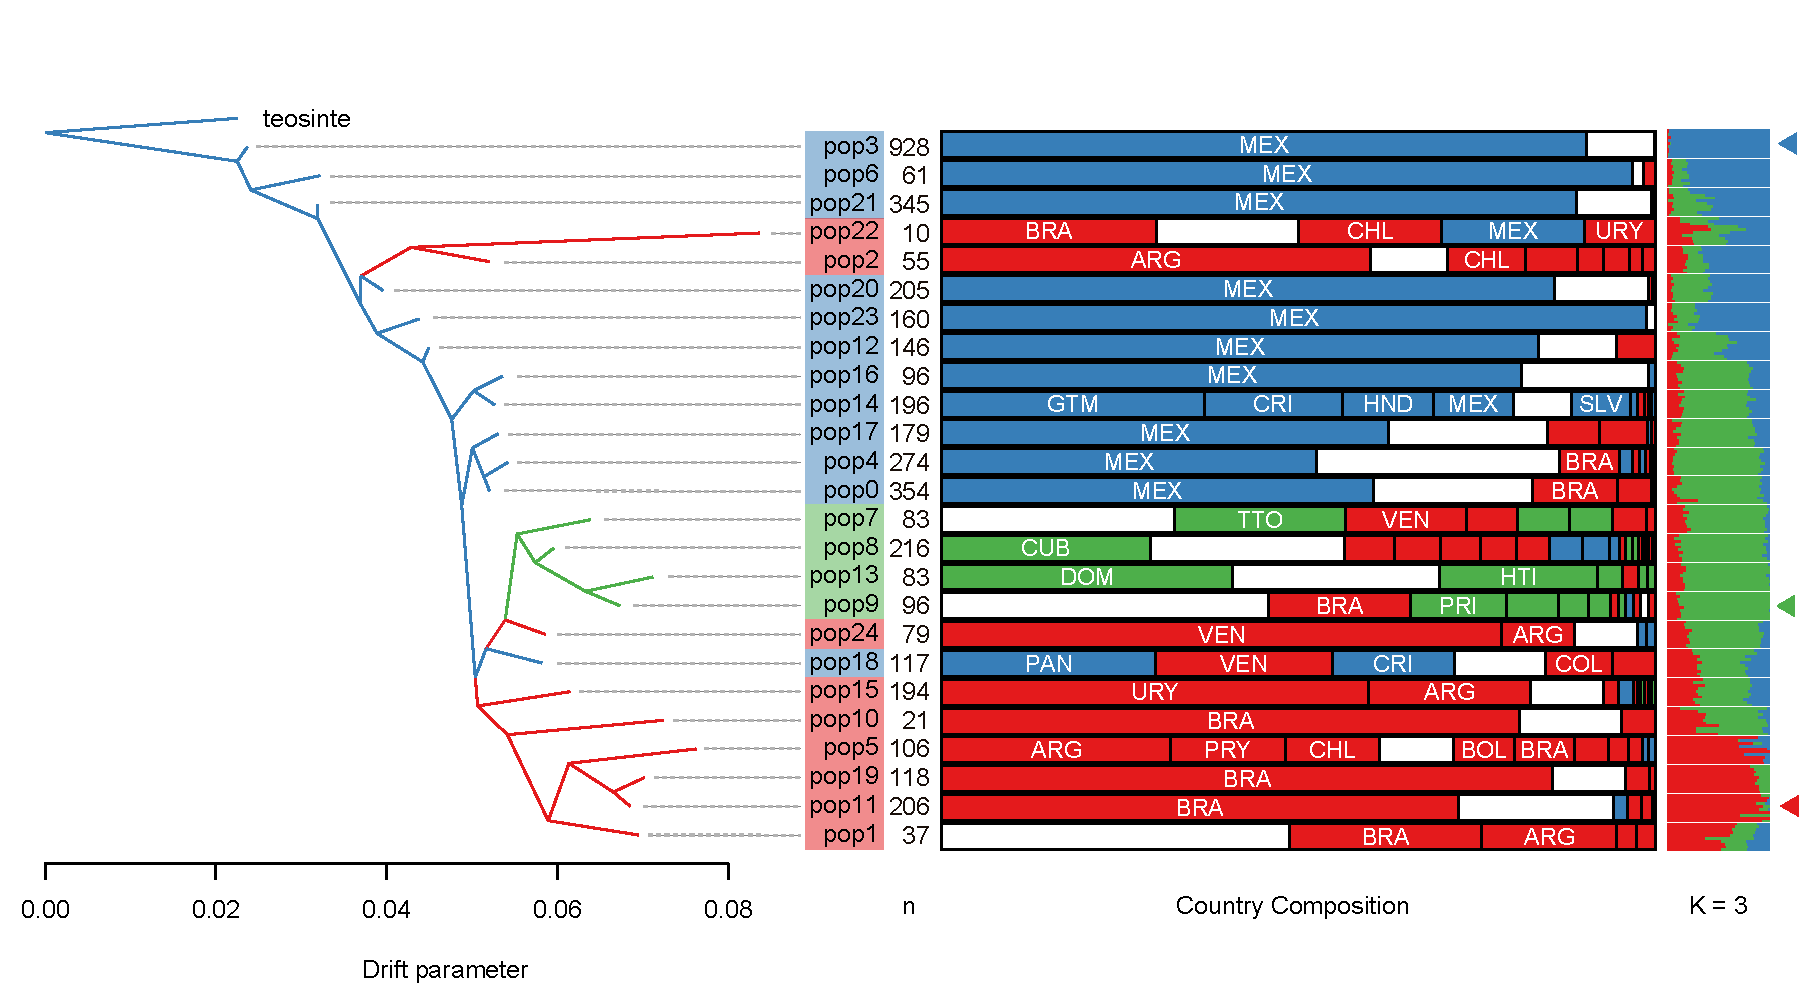
\includegraphics[width=\textwidth]{fig7.pdf}

\caption{\color{Gray} \textbf{Demographic history K = 25}. \textbf{A-F}, This figure is wrapped into the standard floating environment.}

\label{fig7} % \label works only AFTER \caption within figure environment

\end{figure}

\begin{figure}[h] %s state preferences regarding figure placement here

% use to correct figure counter if necessary
%\renewcommand{\thefigure}{2}

\includegraphics[width=\textwidth]{fig8.pdf}

\caption{\color{Gray} \textbf{Population Map}. \textbf{A-F}, This figure is wrapped into the standard floating environment.}

\label{fig8} % \label works only AFTER \caption within figure environment

\end{figure}


\nolinenumbers

\newpage

%This is where your bibliography is generated. Make sure that your .bib file is actually called library.bib
\bibliography{library}

%This defines the bibliographies style. Search online for a list of available styles.
\bibliographystyle{abbrv}

\end{document}

